\documentclass[e4_tp1_main.tex]{subfiles}
\begin{document}

\section{DCM y Eficiencia}


Para llevar el circuito del inciso anterior a modo discontinuo se dismunuy\'o la corriente de salida a $I_o=10mA$.  Para una tensi\'on de salida $V_o=3.3V$ con $\Delta V_o =5\%$, debimos modificar el duty cycle a $D_{real}=0.35$.

\begin{figure}[H]
\centering
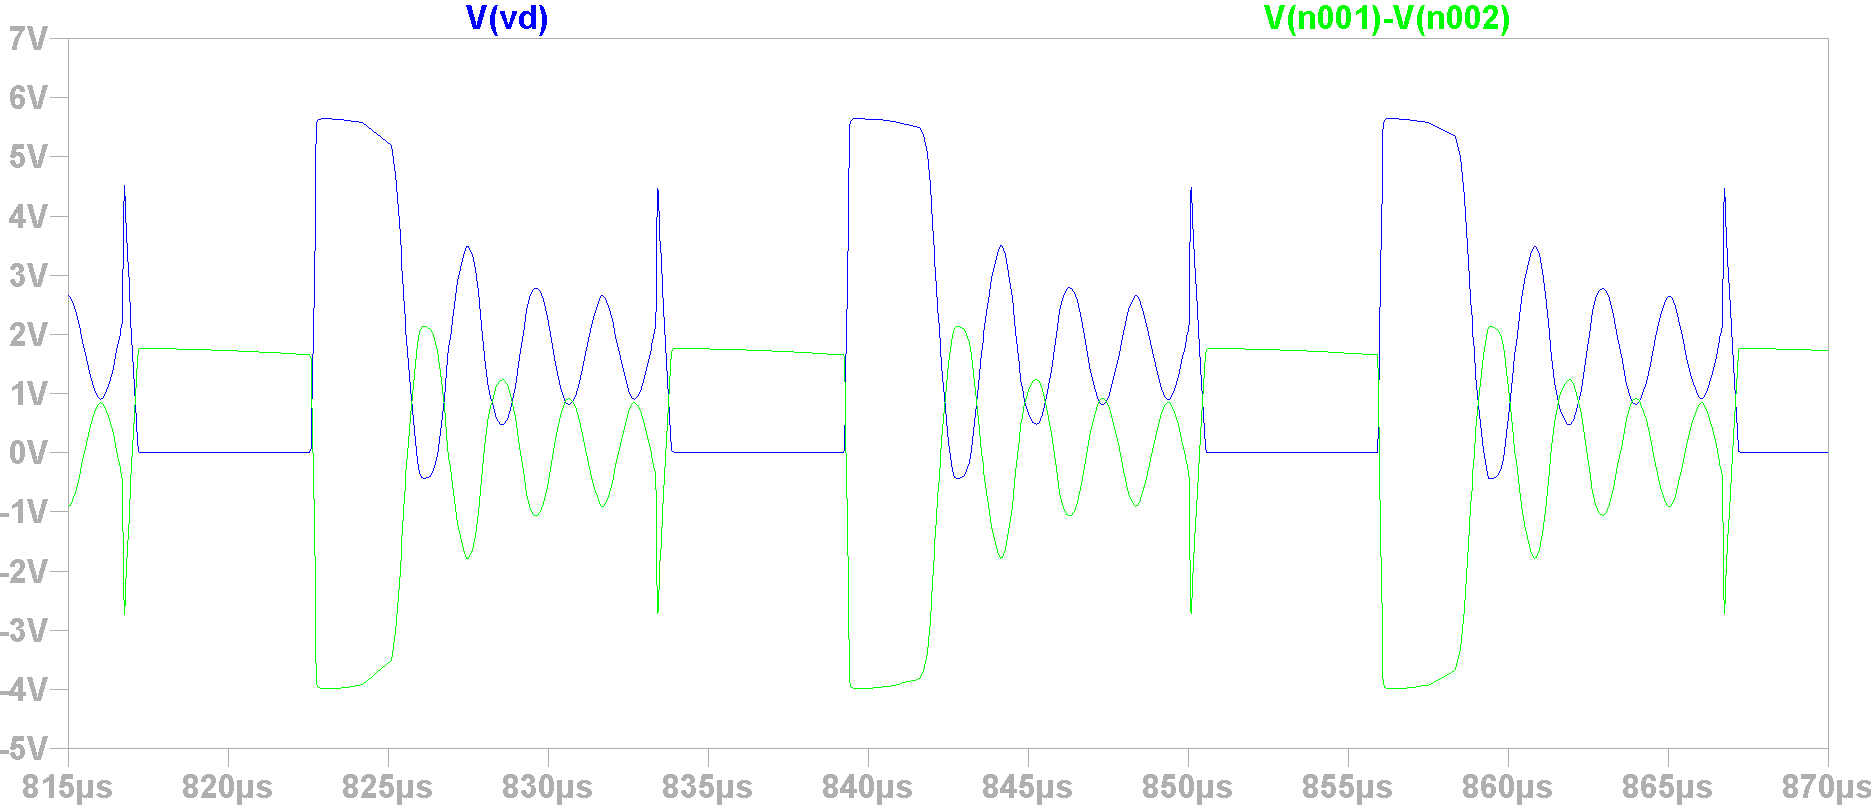
\includegraphics[width=0.7\linewidth]{Imagenes/Punto4/SW&VL}
\caption{Simulación Sw(azul) y VL(verde)}
\end{figure}

\begin{figure}[H]
\centering
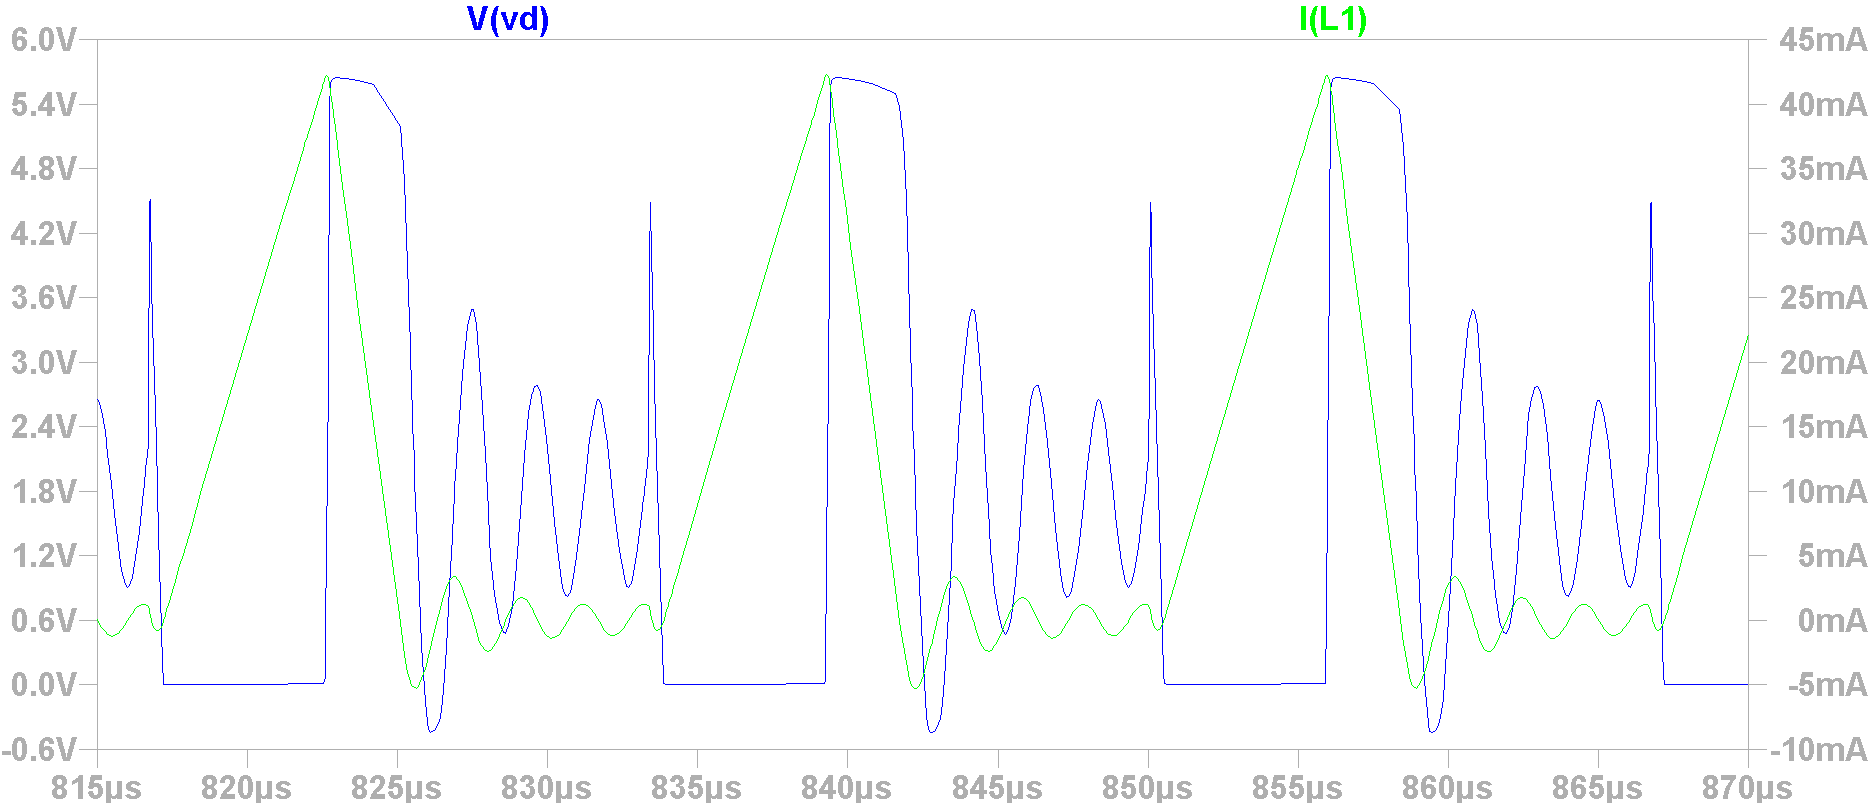
\includegraphics[width=0.7\linewidth]{Imagenes/Punto4/SW&IL}
\caption{Simulación Sw(azul) y IL(verde)}
\end{figure}

\begin{figure}[H]
\centering
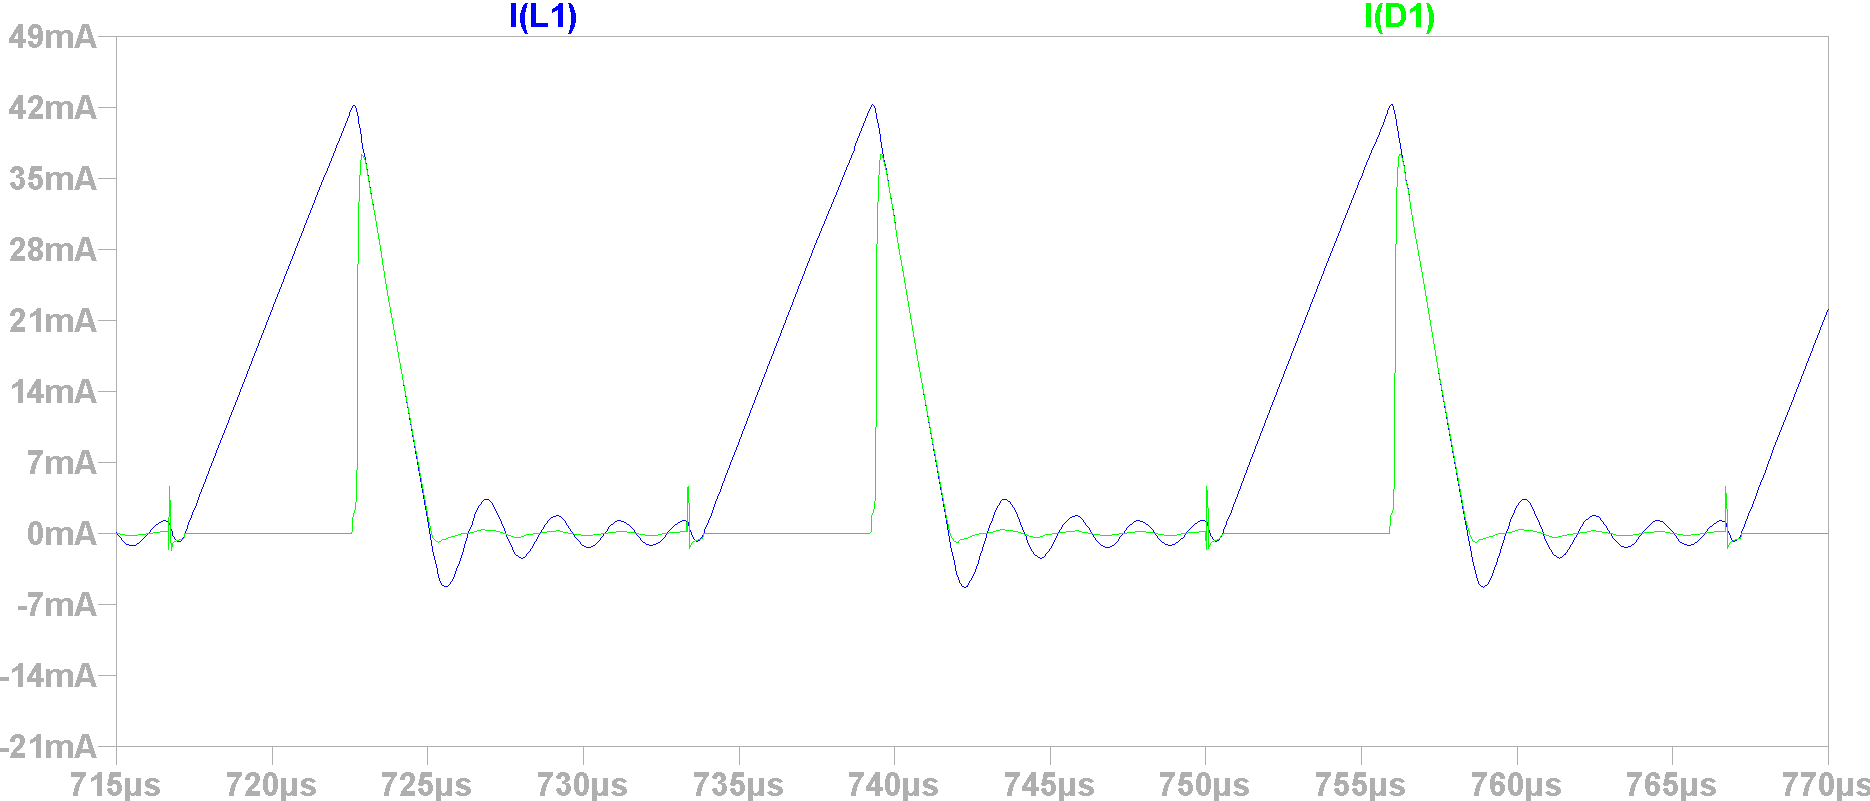
\includegraphics[width=0.7\linewidth]{Imagenes/Punto4/IL&ID}
\caption{Simulación IL(azul) y ID(verde)}
\end{figure}

\begin{figure}[H]
\centering
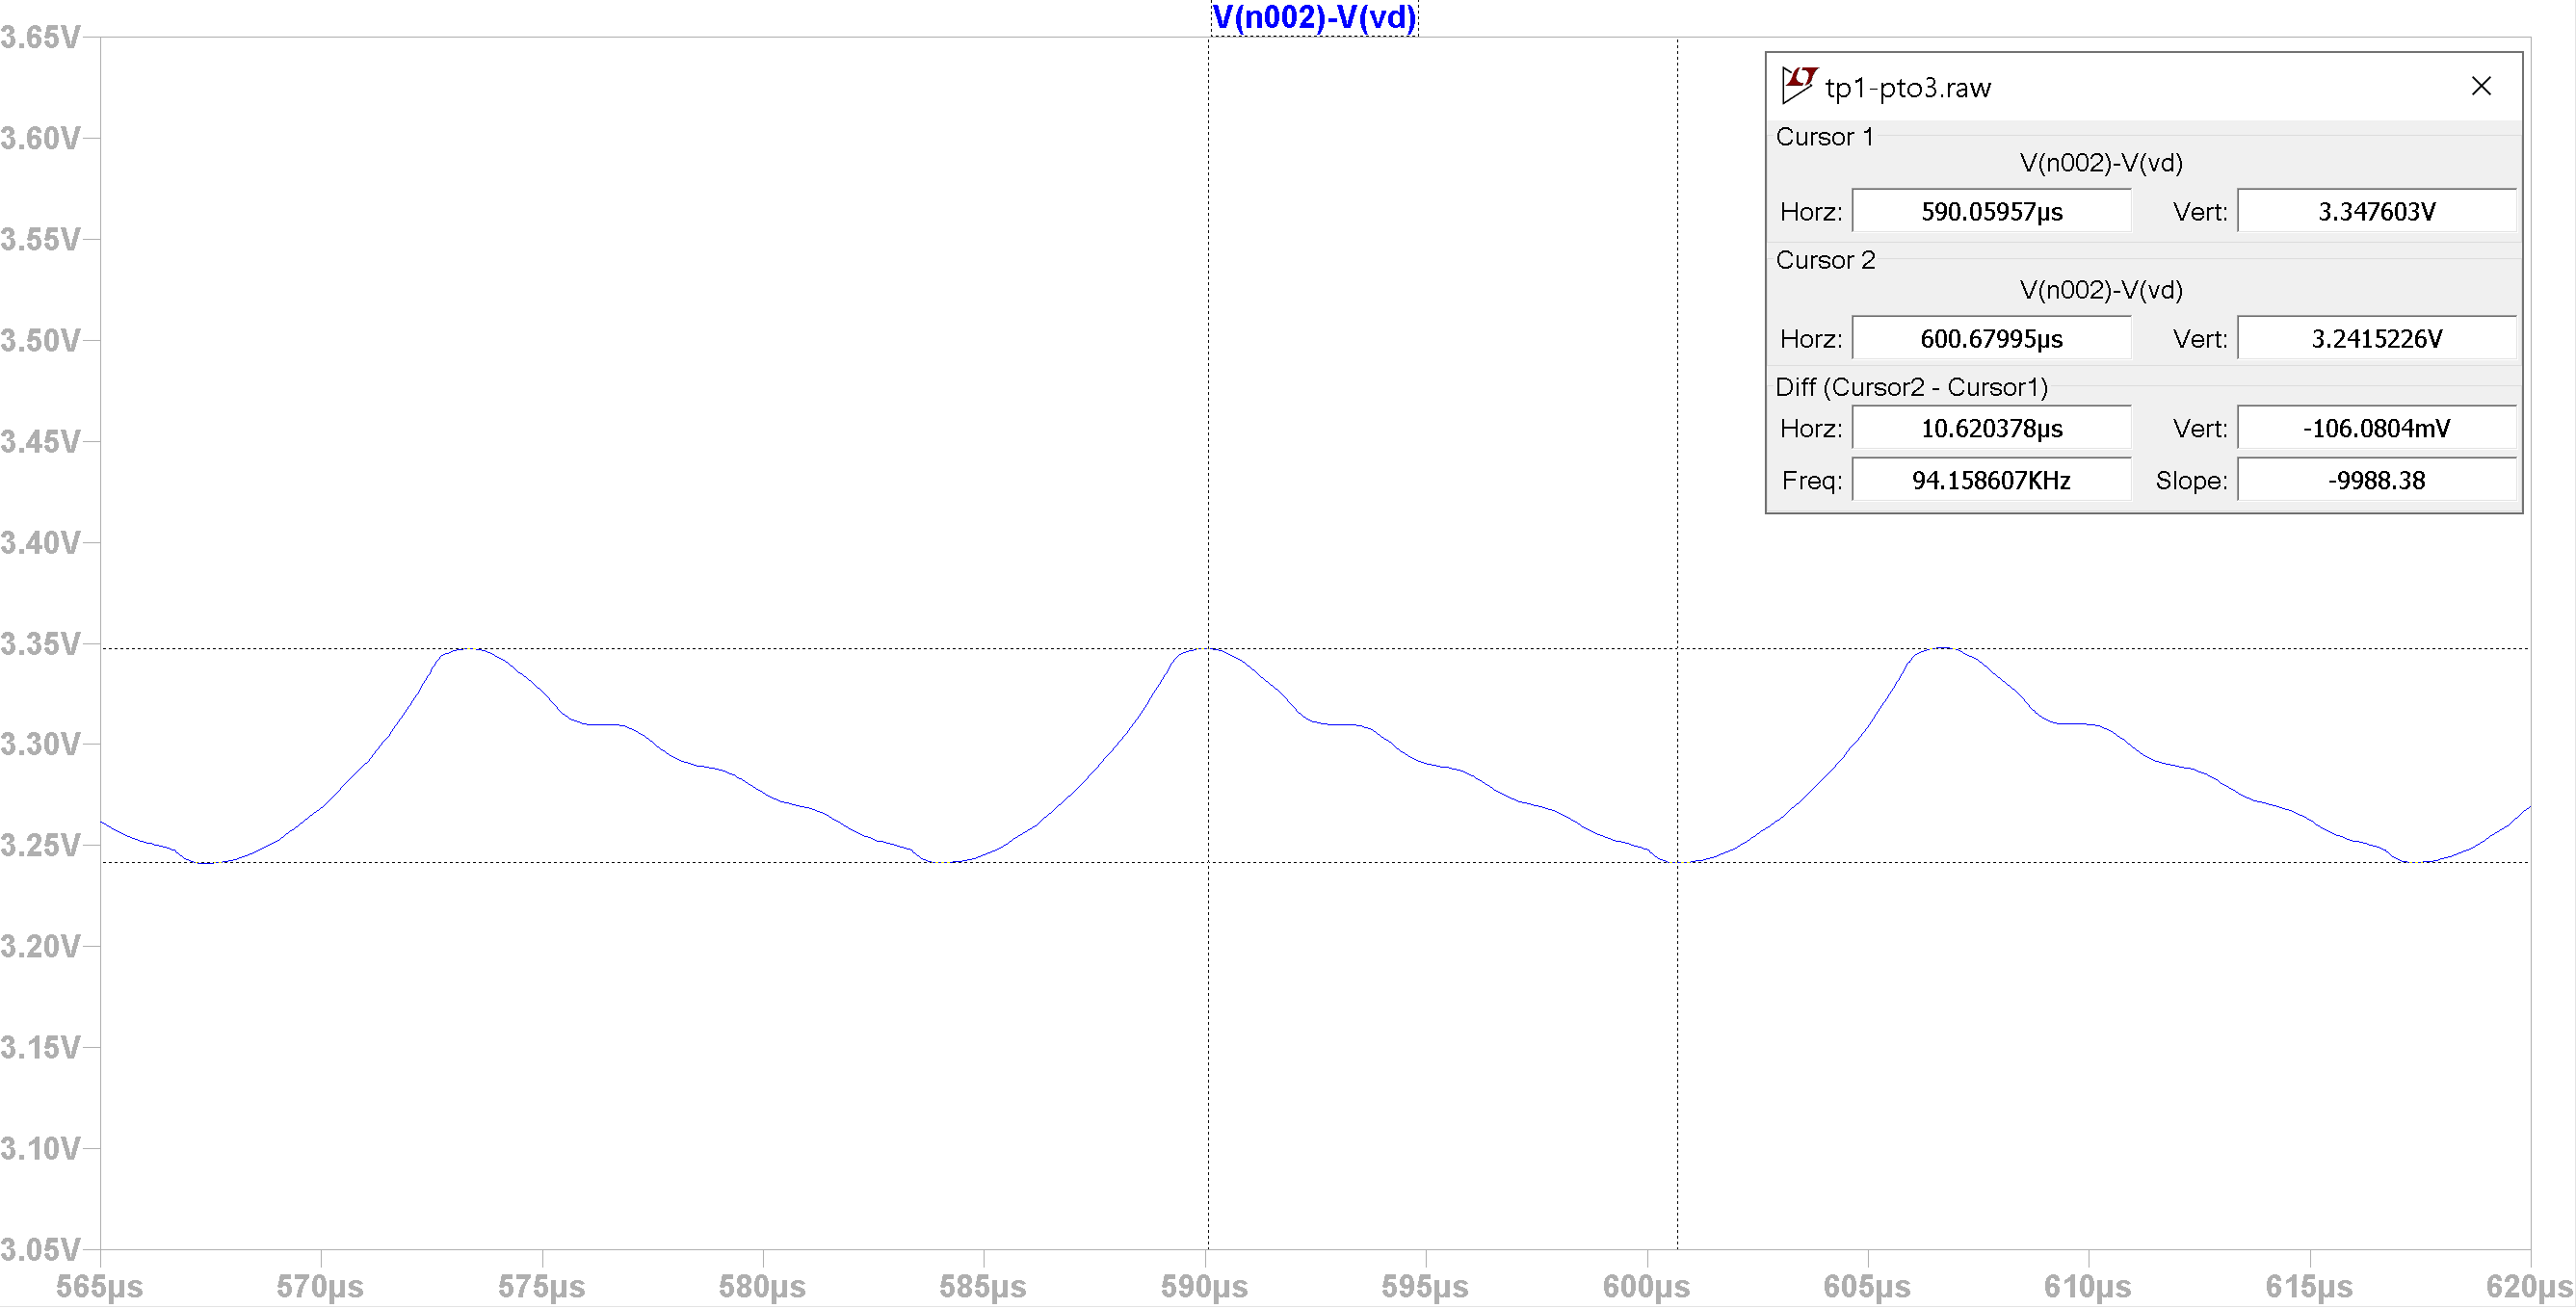
\includegraphics[width=0.7\linewidth]{Imagenes/Punto4/Vo-D=0,35.PNG}
\caption{Simulación $V_o$}
\end{figure}




\newpage
\end{document}